% Preamble
\documentclass[11pt]{PyRollDocs}
\usepackage{textcomp}

\addbibresource{refs.bib}

% Document
\begin{document}

    \title{The Roux Spreading PyRoll Plugin}
    \author{Christoph Renzing}
    \date{\today}

    \maketitle

    This plugin provides a spreading modelling approach with Roux's formula for flat rolling, adapted on groove rolling by an equivalent rectangle approach.


    \section{Model approach}\label{sec:model-approach}

    \subsection{Roux's spread equation}\label{subsec:roux's-spread-equation}

    \textcite{} proposed \autoref{eq:roux} for estimation of spreading in flat rolling.
    Where $h$ and $b$ are height and width of the workpiece with the indices 0 and 1 denoting the incoming respectively the outgoing profile.
    $C_1$ and $C_2$ are parameters introduced by Roux.
    $R$ is the roll radius and $\mu$ is the friction coefficient.


    \begin{equation}
        C_1 = \left( 1 + 5 \left( 0.35 - \frac{\Delta h}{h_0}\right)^2 \right) \sqrt{\frac{h_0}{\Delta h}} -1
        \label{eq:roux-parameter-c1}
    \end{equation}

    \begin{equation}
        C_2 = \left( \frac{b_0}{h_0} - 1 \right) \left( \frac{b_0}{h_0} \right)^{\frac{2}{3}}
        \label{eq:roux-parameter-c2}
    \end{equation}

    \begin{equation}
        b_1 = b_0 + \left( h_0 - h_1 \right) \frac{1}{\left( 1 - \frac{\delta h}{h_0} \right) + \frac{3 C_1}{\left( 2 \frac{R}{h_0} \right)^{\frac{3}{4}}}} \frac{\frac{b_0}{h_0}}{1 + 0.57 C_2}
        \label{eq:roux}
    \end{equation}

    \subsection{Equivalent rectangle approach}\label{subsec:equivalent-rectangle-approach}

    Roux's spreading model~\cite{Roux1939} was originally built for flat rolling.
    A common approach for groove rolling is to calculate some equivalent rectangular profile to be able to use flat rolling models~\cite{Hensel1978, Spittel1984}.
    \autoref{fig:equivalent_rectangle} shows 3 variants of calculating an equivalent rectangle of a profile.

    \begin{figure}
        \centering
        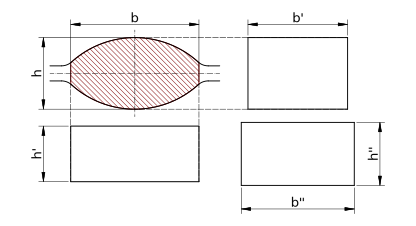
\includegraphics[width=\linewidth]{equivalent_rectangle}
        \caption{Three methods of defining an equivalent rectangle of an oval groove}
        \label{fig:equivalent_rectangle}
    \end{figure}

    The first variant is to keep the width constant and calculate the height $h'$ so that the cross section $A$ is
    equal:

    \[
        h' = \frac{A}{b}
    \]

    The second variant is to keep the height constant and calculate the width $b'$ so that the cross section $A$ is
    equal:

    \[
        b' = \frac{A}{h}
    \]

    Both represent the geometry of the profile poorly.
    A better way is to keep the aspect ratio equal as propose by \textcite{Spittel1984}:

    \[
        h'' = \sqrt{\frac{A h}{b}}
    \]

    \[
        b'' = \sqrt{\frac{A b}{h}}
    \]

    This variant is used in the current implementation.
    So $h$ and $b$ in Roux's model are replaced with $h''$ and $b''$.
    In the end, $b_1$ can be obtained from $b_1''$ by:

    \[
        b_1 = \frac{b_1'' h_1}{h_1''}
    \]


    \section{Usage instructions}\label{sec:usage-instructions}

    The plugin can be loaded under the name \texttt{pyroll\_roux\_spreading}.

    An implementation of the \lstinline{width_change} hook on \lstinline{RollPass} is provided,
    calculating the spread using the equivalent rectangle approach and Roux's model.

    Several additional hooks on \lstinline{RollPass} are defined, which are used in spread calculation, as listed in \autoref{tab:hookspecs}.
    Base implementations of them are provided, so it should work out of the box.
    For \lstinline{marini_parameter_a} and \lstinline{marini_parameter_b} the equations~\ref{eq:roux-parameter-c1} and~\ref{eq:roux-parameter-c2} are implemented.
    Friction coefficient can be adjusted individually.
    Provide your own hook implementations or set attributes on the \lstinline{RollPass} instances to alter the spreading behavior.

    \begin{table}
        \centering
        \caption{Hooks specified by this plugin. Symbols as in \autoref{eq:roux}.}
        \label{tab:hookspecs}
        \begin{tabular}{ll}
            \toprule
            Hook name                     & Meaning                                      \\
            \midrule
            \texttt{roux\_parameter\_c1}   & Parameter $C_1$ of Roux's spreading equation \\
            \texttt{roux\_parameter\_c2}   & Parameter $C_2$ of Roux's spreading equation \\
            \bottomrule
        \end{tabular}
    \end{table}

    \printbibliography

\end{document}